\documentclass[12pt]{article}
\usepackage[utf8]{inputenc} % Sin el guion
\usepackage[T1]{fontenc}    % Ayuda a que las tildes se copien bien del PDF
\usepackage[spanish]{babel}
\usepackage{amsmath}
\usepackage{amssymb}
\usepackage{geometry}
\usepackage[backend=biber,style=numeric]{biblatex}
\usepackage{csquotes}
\bibliography{referencias}
\geometry{margin=1in}
\usepackage{listings}
\usepackage{xcolor}

\usepackage{graphicx}
\usepackage{float}      % opcional, para usar [H]
\usepackage{hyperref}   % opcional, para referencias clickeables

\lstset{
    language=Python,
    basicstyle=\ttfamily\footnotesize,
    keywordstyle=\color{blue},
    commentstyle=\color{gray},
    stringstyle=\color{black},
    numbers=left,
    numberstyle=\tiny,
    frame=single,
    rulecolor=\color{black},
    breaklines=true,
    showstringspaces=false
}

\title{Actividad 2}
\author{Ing. Isaias Garcia Zanella}
\date{\today}

\begin{document}

\maketitle

\section{Introducción}
En esta actividad se realizará una investigación más profunda sobre las 
mediciones de distancia que existen y también se realizará una práctica con Python para la imputación de datos en bases de datos (B.D.) con datos faltantes, 
además de la identificación de datos atípicos y la codificación y normalización de datos para su posterior uso, ya sea en modelos de Machine Learning o en interpretaciones gráficas.

\section{Marco Teórico}
\subsection{Medidas de Distancia}
En muchos algoritmos de IA, el cálculo de la distancia es un elemento
crucial para calcular la similaridad entre conjuntos de vectores.~\cite{De0a100enIA}

Esto es importante para algoritmos de clustering, clasificación, reducción de dimensionalidad, entre otros.
Existen varias medidas de distancia, cada una con sus propias características y aplicaciones. A continuación, se describen algunas de las medidas de distancia más comunes:

\subsubsection{Distancia Euclidiana}
La distancia euclidiana está basada en la distancia bidimensional entre dos vectores; es decir, la 
distancia entre dos puntos como si se dibujara una línea con una regla de un punto al otro. Esta es una de las distancias que
más se utiliza en algoritmos de aprendizaje automático.

Específicamente, si se tienen dos puntos $(x_1, y_1)$ y $(x_2, y_2)$, la distancia euclidiana puede ser calculada usando la fórmula:
\begin{equation}
d = \sqrt{(x_2 - x_1)^2 + (y_2 - y_1)^2}
\end{equation}
~\cite{De0a100enIA}

\subsubsection{Distancia de Manhattan}
La distancia de Manhattan es también llamada distancia del taxi (o <<Taxicab>>). Se puede entender mejor esta distancia
como si alguien estuviera manejando por una ciudad. Para calcular la distancia de Manhattan entre dos puntos, se suman las distancias absolutas como se muestra en la siguiente ecuación:
\begin{equation}
    D = \sum_{i = 1}^{n} |x_i - y_i|
\end{equation}
~\cite{De0a100enIA}

\subsubsection{Distancia de Chebyshev}
La distancia de Chebyshev también es muy utilizada en algoritmos de aprendizaje automático.
Se conoce comúnmente como distancia del ajedrez. En el ajedrez, cada pieza se mueve de manera diferente en el tablero. En este sentido, la
distancia de Chebyshev se puede interpretar como el número de movimientos en los que el rey puede llegar desde su posición inicial a cierta posición en el tablero.

La representación matemática de la distancia de Chebyshev se muestra en la siguiente ecuación:
\begin{equation}
    D_{Cheb} = \max (|x_2 - x_1|, |y_2 - y_1|)
\end{equation}
~\cite{De0a100enIA}

\subsubsection{Distancia de Hamming}
La distancia de Hamming mide cuántos elementos son diferentes entre dos secuencias del mismo tamaño. Es como contar
los “errores” o diferencias entre dos cadenas de datos.

Matemáticamente se expresa por medio de la siguiente ecuación:
\begin{equation}
    d_{p,q} = \sum_{i=1}^{n} \delta(p_i, q_i)
\end{equation}

Donde:
\begin{itemize}
    \item \textit{p} y \textit{q} son dos cadenas o vectores del tamaño \textit{n}.
    \item $\delta(p_i, q_i)$ es 1 si $p_i \neq q_i$, y 0 si $p_i = q_i$.
\end{itemize}
~\cite{De0a100enIA}

\subsubsection{Distancia de Bhattacharyya}
La distancia de Bhattacharyya mide la similitud entre dos distribuciones de probabilidad. Se utiliza principalmente
para evaluar qué tan “parecidas” son dos conjuntos de datos representados como distribuciones.

Matemáticamente, se puede expresar como en la ecuación siguiente:
\begin{equation}
    D_B(p, q) = -\ln \left( \sum_{i=1}^{n} \sqrt{p_i \cdot q_i} \right)
\end{equation}

Donde:
$p_i$ y $q_i$ son las probabilidades asociadas a la i-ésima categoría o intervalo en las distribuciones $p$ y $q$.

La suma $\left( \sum_{i=1}^{n} \sqrt{p_i \cdot q_i} \right)$ se conoce como el coeficiente de Bhattacharyya. Si las distribuciones son idénticas, el coeficiente será 1 y la distancia es 0. Cuanto más diferentes sean, mayor será la distancia.
~\cite{De0a100enIA}

\subsubsection{Distancia de Jaccard}
La \textbf{distancia de Jaccard} mide cuán diferentes son dos conjuntos al comparar los elementos que tienen en común frente a los que no. Es una métrica basada en el concepto de intersección y unión de conjuntos.

Matemáticamente, se puede expresar de la siguiente manera:
\begin{equation}
    d_J(A, B) = 1 - \frac{|A \cap B|}{|A \cup B|}
\end{equation}

Donde:
\begin{itemize}
    \item $A$ y $B$ son dos conjuntos.
    \item $|A \cap B|$ es el número de elementos que están en ambos conjuntos (intersección).
    \item $|A \cup B|$ es el número de elementos que están en al menos uno de los conjuntos (unión).
\end{itemize}
~\cite{De0a100enIA}

\subsubsection{Distancia de Mahalanobis}
La \textbf{distancia de Mahalanobis} es una métrica que mide la distancia entre un punto y un conjunto de datos, teniendo en cuenta la correlación y la variabilidad de las variables. A diferencia de la distancia euclidiana, no asume que todas las variables tienen la misma importancia o escala,
sino que ajusta la medición según cómo están distribuidas las variables y cómo se relacionan entre sí.

La distancia de Mahalanobis entre un punto $p$ y un conjunto de datos representado por el vector promedio $\mu$ es:
\begin{equation}
    d(p,q) = \sqrt{(p-\mu)^T S^{-1} (p-\mu)}
\end{equation} 

Donde:
\begin{itemize}
    \item $p$: es el punto en cuestión (un vector de características).
    \item $\mu$: es el vector promedio (media) de los datos.
    \item $S$: es la matriz de covarianza de los datos.
    \item $S^{-1}$: es la inversa de la matriz de covarianza.
\end{itemize}

Esta medida de distancia tiene las siguientes aplicaciones:
\begin{itemize}
    \item \textbf{Detección de anomalías}: Detectar valores atípicos en conjuntos de datos.
    \item \textbf{Clasificación estadística}: Clasificar puntos en función de su cercanía a un grupo con una distribución conocida.
    \item \textbf{Análisis multivariable}: Comparar observaciones en datasets donde las variables tienen diferentes escalas y están correlacionadas.
\end{itemize}

Esta medida de distancia también tiene las siguientes limitaciones:
\begin{itemize}
    \item \textbf{Requiere matriz de covarianza}: Si el número de observaciones es menor que el número de variables, la matriz de covarianza puede ser singular y no invertible.
    \item \textbf{Supone distribución normal}: La distancia de Mahalanobis funciona mejor si las variables siguen una distribución normal multivariada. 
    \item \textbf{Sensibilidad a valores atípicos}: Los outliers pueden distorsionar la matriz de covarianza, afectando la medición de distancias.
    \item \textbf{Costo computacional}: Calcular la inversa de la matriz de covarianza puede ser difícil en datasets grandes o de alta dimensión.
\end{itemize}
~\cite{De0a100enIA}

\subsubsection{Distancia de Bray-Curtis}
La \textbf{distancia de Bray-Curtis} es una medida utilizada para comparar la diferencia relativa entre dos conjuntos de datos, especialmente cuando los datos
representan cantidades (como conteos o proporciones). Esta métrica es muy popular en estudios ecológicos y análisis de comunidades, donde se quiere medir la disimilitud entre dos muestras basándose en sus composiciones.

La distancia de Bray-Curtis entre dos puntos $p$ y $q$ en un espacio de $n$ dimensiones es:
\begin{equation}
        d(p,q) =\frac{\sum_{i=1}^{n} | p_i - q_i|}{\sum_{i=1}^{n} (p_i + q_i)}
\end{equation}

Donde:
\begin{itemize}
    \item $p_i$ y $q_i$ son los valores para la $i$-ésima variable.
    \item El numerador es la suma de las diferencias absolutas entre los valores de cada dimensión.
    \item El denominador es la suma total de los valores combinados.
\end{itemize}

El valor de $d(p,q)$ está entre 0 y 1:
\begin{itemize}
    \item \textbf{0} significa que los dos conjuntos son completamente iguales.
    \item \textbf{1} indica que no comparten ningún elemento en común.
\end{itemize}
~\cite{De0a100enIA}

\subsubsection{Distancia de Canberra} 
La distancia de Canberra es una medida de disimilitud que compara dos puntos en un espacio multidimensional, poniendo más peso a las diferencias en dimensiones pequeñas.
Es especialmente útil cuando se quiere resaltar diferencias relativas en valores cercanos a cero.

La distancia de Canberra entre dos puntos $p$ y $q$ con $n$ dimensiones es:
\begin{equation}
    d(p,q) = \sum_{i=1}^{n} \frac{|p_i - q_i|}{|p_i| + |q_i|}
\end{equation} 

Donde:
\begin{itemize}
    \item $p_i$ y $q_i$ son los valores en la dimensión $i$.
    \item El numerador mide la diferencia absoluta.
    \item El denominador normaliza esta diferencia en función de la suma de los valores.
\end{itemize}

~\cite{De0a100enIA}

% \subsection{Datos Faltantes}
\subsection{Datos Faltantes}

En el análisis de datos, los datos faltantes (missing data) son valores que no se encuentran registrados en una o más variables del conjunto de datos. La presencia de datos faltantes puede afectar significativamente el desempeño de los modelos estadísticos y de aprendizaje automático, generando sesgos o reduciendo la precisión de las predicciones~\cite{little2019missing}.

Los datos faltantes se clasifican generalmente en tres categorías~\cite{little2019missing}:

\begin{itemize}
    \item \textbf{MCAR (Missing Completely At Random)}: Los datos faltan completamente al azar y su ausencia no depende de ninguna variable observada o no observada.
    \item \textbf{MAR (Missing At Random)}: La ausencia depende de variables observadas, pero no del valor faltante en sí.
    \item \textbf{MNAR (Missing Not At Random)}: La ausencia depende del propio valor faltante.
\end{itemize}

El tratamiento adecuado de los datos faltantes es fundamental para garantizar la validez del análisis posterior~\cite{hastie2009elements}.
% \subsection{Datos Atípicos (IQR)}
\subsection{Datos Atípicos (IQR)}

Los datos atípicos (outliers) son observaciones que se alejan significativamente del comportamiento general del conjunto de datos. Estos pueden surgir debido a errores de medición, errores de registro o variabilidad natural del fenómeno estudiado~\cite{tukey1977exploratory}.

Una técnica común para detectar valores atípicos es el método del rango intercuartílico (IQR, Interquartile Range), propuesto en el contexto del análisis exploratorio de datos~\cite{tukey1977exploratory}. El IQR se define como:

\begin{equation}
IQR = Q_3 - Q_1
\end{equation}

donde $Q_1$ es el primer cuartil (percentil 25) y $Q_3$ es el tercer cuartil (percentil 75).

Un valor se considera atípico si cumple:

\begin{equation}
x < Q_1 - 1.5(IQR) \quad \text{o} \quad x > Q_3 + 1.5(IQR)
\end{equation}

Este método es ampliamente utilizado debido a su simplicidad y robustez frente a distribuciones no normales~\cite{han2011data}.
\subsection{Imputación}

La imputación es el proceso mediante el cual se reemplazan los valores faltantes por estimaciones plausibles, con el objetivo de preservar la mayor cantidad de información posible sin introducir sesgos significativos~\cite{little2019missing}.

Existen diferentes métodos de imputación~\cite{hastie2009elements, james2021introduction}:

\begin{itemize}
    \item \textbf{Imputación por media, mediana o moda}: Sustituye los valores faltantes por estadísticas descriptivas.
    \item \textbf{Imputación por regresión}: Utiliza modelos estadísticos para estimar valores faltantes.
    \item \textbf{K-Nearest Neighbors (KNN)}: Imputa valores basándose en observaciones similares.
    \item \textbf{Imputación múltiple}: Genera múltiples conjuntos de datos imputados para reducir la incertidumbre.
\end{itemize}

La elección del método depende del tipo de variable y del mecanismo de ausencia de los datos~\cite{little2019missing}.
% \subsection{Codificación}
\subsection{Codificación}

La codificación es el proceso de transformar variables categóricas en representaciones numéricas para que puedan ser utilizadas por algoritmos de aprendizaje automático~\cite{han2011data}.

Algunos métodos comunes incluyen~\cite{james2021introduction}:

\begin{itemize}
    \item \textbf{Label Encoding}: Asigna un número entero a cada categoría.
    \item \textbf{One-Hot Encoding}: Crea una variable binaria por cada categoría.
    \item \textbf{Target Encoding}: Codifica las categorías según la variable objetivo.
\end{itemize}

La selección del método adecuado depende del tipo de modelo y de la naturaleza de los datos~\cite{hastie2009elements}.
% \subsection{Normalización}
\subsection{Normalización}

La normalización es una técnica de preprocesamiento que consiste en escalar los datos numéricos para que se encuentren dentro de un rango específico o tengan propiedades estadísticas determinadas~\cite{han2011data}.

Algunos métodos comunes son~\cite{james2021introduction}:

\begin{itemize}
    \item \textbf{Min-Max Scaling}:
    \begin{equation}
    x' = \frac{x - x_{min}}{x_{max} - x_{min}}
    \end{equation}

    \item \textbf{Estandarización (Z-score)}:
    \begin{equation}
    x' = \frac{x - \mu}{\sigma}
    \end{equation}
\end{itemize}

La normalización es especialmente importante en algoritmos basados en distancia, como KNN, SVM o métodos de clustering, ya que evita que variables con mayor escala dominen el cálculo~\cite{hastie2009elements}.

\section{Materiales y Métodos}

\subsection{Materiales}

Para el desarrollo de la presente actividad se utilizó el siguiente equipo de cómputo y herramientas de software:

\begin{itemize}
    \item \textbf{Equipo:} Laptop HP Victus.
    \item \textbf{Procesador:} AMD Ryzen 7000 Series.
    \item \textbf{Tarjeta gráfica:} NVIDIA GeForce RTX 4050.
    \item \textbf{Lenguaje de programación:} Python.
    \item \textbf{Entorno de desarrollo:} Visual Studio Code (VS Code).
    \item \textbf{Bibliotecas utilizadas:} Pandas (para manejo de datos y detección de valores nulos).
\end{itemize}

El equipo permitió ejecutar los algoritmos de análisis de datos, detección de valores atípicos, imputación, codificación y normalización de manera eficiente. Visual Studio Code se empleó como entorno de desarrollo integrado (IDE) para la escritura, ejecución y depuración del código, facilitando la organización del proyecto y la gestión de librerías.

\subsection{Métodos}

El procesamiento de datos se realizó mediante funciones programadas en Python, utilizando la biblioteca Pandas para el manejo de valores nulos.

\subsubsection{Detección de Datos Faltantes}

Se implementó la siguiente función para calcular el porcentaje de valores faltantes:

\begin{lstlisting}[caption=Funcion para calcular porcentaje de datos faltantes, label=lst:missing]
def get_empty_Data(data_list):
    empty_count = sum(1 for x in data_list if pd.isna(x))
    porcentaje = (empty_count / len(data_list)) * 100
    return porcentaje
\end{lstlisting}

La función cuenta los valores nulos y calcula su proporción respecto al total de datos.

\subsubsection{Detección de Valores Atípicos (IQR)}

Para la detección de valores atípicos se implementó el siguiente algoritmo basado en el rango intercuartílico:

\begin{lstlisting}[caption=Deteccion de valores atipicos mediante IQR, label=lst:iqr]
def calcular_estadisticas_outliers(data_list):
    if not data_list:
        return None

    data_ordenada = sorted(data_list)

    def get_percentile(data, percentile):
        k = (len(data) - 1) * percentile
        f = int(k)
        c = k - f
        if f + 1 < len(data):
            return data[f] + (data[f+1] - data[f]) * c
        else:
            return data[f]

    q1 = get_percentile(data_ordenada, 0.25)
    q3 = get_percentile(data_ordenada, 0.75)
    iqr = q3 - q1

    limite_inferior = q1 - 1.5 * iqr
    limite_superior = q3 + 1.5 * iqr

    outliers = [x for x in data_list 
                if x < limite_inferior or x > limite_superior]

    return {
        "q1": q1,
        "q3": q3,
        "iqr": iqr,
        "limite_inf": limite_inferior,
        "limite_sup": limite_superior,
        "outliers": outliers
    }
\end{lstlisting}

El método calcula los cuartiles, el IQR y determina los límites inferior y superior para identificar valores atípicos.

\subsubsection{Métodos de Imputación}

% \paragraph{Imputación por Media}

\begin{lstlisting}[caption=Imputacion por media, label=lst:media]
def imputacion_media(data_list):
    media = get_mean(data_list)
    data_imputada = [media if pd.isna(x) else x 
            for x in data_list]
    cambios = []
    for i, x in enumerate(data_list):
        if pd.isna(x):
            cambios.append({"indice": i, 
                            "valor_nuevo": media})

    return data_imputada, cambios
\end{lstlisting}

% \paragraph{Imputación por Vecinos Más Cercanos (KNN)}

\begin{lstlisting}[caption=Imputacion por vecinos mas cercanos (KNN), label=lst:knn]
def imputacion_knn(data_list, k=3):
    data_imputada = []
    cambios = []

    for i, x in enumerate(data_list):
        if pd.isna(x):
            vecinos = []

            for j in range(i-1, max(i-k-1, -1), -1):
                if not pd.isna(data_list[j]):
                    vecinos.append(data_list[j])
                if len(vecinos) >= k:
                    break

            for j in range(i+1, min(i+k+1, len(data_list))):
                if not pd.isna(data_list[j]):
                    vecinos.append(data_list[j])
                if len(vecinos) >= k:
                    break

            if vecinos:
                nuevo_valor = sum(vecinos) / len(vecinos)
                data_imputada.append(nuevo_valor)
                cambios.append({
                    "indice": i,
                    "valor_nuevo": nuevo_valor,
                    "vecinos_usados": vecinos.copy()
                })
            else:
                data_imputada.append(x)
        else:
            data_imputada.append(x)

    return data_imputada, cambios
\end{lstlisting}

% \subsubsection{Codificación One-Hot}
\begin{lstlisting}[caption=Codificacion One-Hot, label=lst:onehot]
def codificacion_one_hot(data_list):
    categorias = sorted(set(x for x in data_list 
                            if str(x).lower() != 'nan'))
    codificacion = {cat: [1 if x == cat else 0 
                          for x in data_list] 
                    for cat in categorias}
    return codificacion
\end{lstlisting}

% \subsubsection{Normalización Min-Max}

\begin{lstlisting}[caption=Normalizacion Min-Max, label=lst:minmax]
def normalizacion_min_max(data_list):
    min_val = get_min_value(data_list)
    max_val = get_max_value(data_list)

    if max_val == min_val:
        return [0.5 for _ in data_list]

    return [(x - min_val) / (max_val - min_val) 
            if not pd.isna(x) else x 
            for x in data_list]
\end{lstlisting}

El procesamiento de datos se realizó mediante funciones programadas en Python. Se implementaron algoritmos para detectar datos faltantes, identificar valores atípicos, aplicar métodos de imputación, realizar codificación de variables categóricas y normalizar los datos numéricos.

% \section{Resultados y Discusión}

% Para la observación y análisis de los datos se utilizó la base de datos disponible en la plataforma Kaggle titulada \textit{``Diabetes Dataset with Missing Value for Practice''}. 

% Este conjunto de datos fue seleccionado debido a que contiene valores faltantes de manera intencional, lo que permite aplicar y evaluar los métodos de imputación, detección de valores atípicos, codificación y normalización desarrollados en la sección anterior.

% El conjunto de datos puede consultarse en el siguiente enlace:

% \url{https://www.kaggle.com/datasets/bhavyamotiyani/diabetes-dataset-with-missing-value-for-practice}

% % \text{Con la columna con la que trabajaremos para los resultados serian con la columna Skin_Fold.}
% Con el objetivo de evaluar el impacto del método de imputación KNN sobre la estructura estadística de la variable analizada, se realizó una comparación de densidades mediante la estimación Kernel (KDE), contrastando los valores originales (sin datos faltantes) con los valores obtenidos después de la imputación.

% \begin{figure}[H]
%     \centering
%     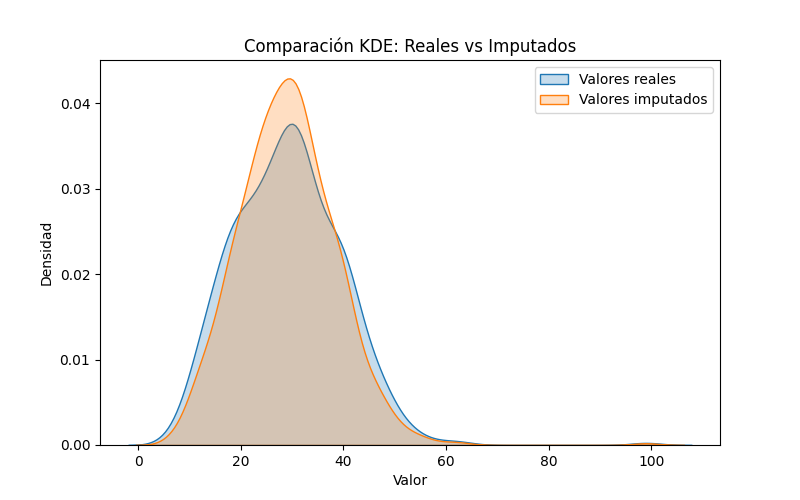
\includegraphics[width=0.7\linewidth]{../Imagenes/Tarea2/Validacion_Original_Imputacion.png}
%     \caption{omparación de densidad (KDE) entre valores originales e imputados mediante KNN.}
%     \label{fig:normalizacion}
% \end{figure}
% Como se observa en la Figura~\ref{fig:kde_knn}, ambas curvas presentan una superposición considerable, lo que indica que el método KNN preserva adecuadamente la forma general de la distribución. No se aprecia un desplazamiento significativo del pico principal ni alteraciones notables en las colas de la distribución.

% A diferencia de la imputación por media, el método KNN genera valores basados en el promedio de los vecinos más cercanos, lo que permite mantener la estructura local de los datos. Esta característica evita la concentración artificial de valores en un punto específico y contribuye a conservar la variabilidad original de la variable.

% Asimismo, no se detecta la generación de valores atípicos adicionales ni una modificación evidente del rango de los datos, lo que sugiere que la imputación no introduce sesgos estadísticos relevantes.

% En consecuencia, los resultados obtenidos indican que el método KNN resulta adecuado para este conjunto de datos, ya que minimiza la distorsión en la distribución original y mantiene las propiedades estadísticas fundamentales de la variable analizada.

\section{Resultados y Discusión}

Para la observación y análisis de los datos se utilizó la base de datos disponible en la plataforma Kaggle titulada \textit{``Diabetes Dataset with Missing Value for Practice''}. 

Este conjunto de datos fue seleccionado debido a que contiene valores faltantes de manera intencional, lo que permite aplicar y evaluar los métodos de imputación, detección de valores atípicos, codificación y normalización desarrollados en la sección anterior.

El conjunto de datos puede consultarse en el siguiente enlace:

\url{https://www.kaggle.com/datasets/bhavyamotiyani/diabetes-dataset-with-missing-value-for-practice}

Para el análisis presentado en esta sección se trabajó específicamente con la columna \texttt{Skin\_Fold}, ya que esta variable contiene valores faltantes y resulta adecuada para evaluar el impacto de los métodos de imputación y normalización.

\subsection{Imputación de Datos mediante KNN}

Para el tratamiento de valores faltantes en la variable \texttt{Skin\_Fold} se empleó el método de los vecinos más cercanos (KNN), el cual sustituye cada valor ausente con base en los valores más próximos dentro del conjunto de datos. Este enfoque permite preservar la estructura local y la variabilidad original de la variable, evitando concentraciones artificiales en un único valor.

Con el fin de evaluar el impacto de la imputación, se realizó una comparación de densidades utilizando estimación Kernel (KDE), contrastando la distribución de los valores originales con la distribución obtenida tras la imputación.

\begin{figure}[H]
    \centering
    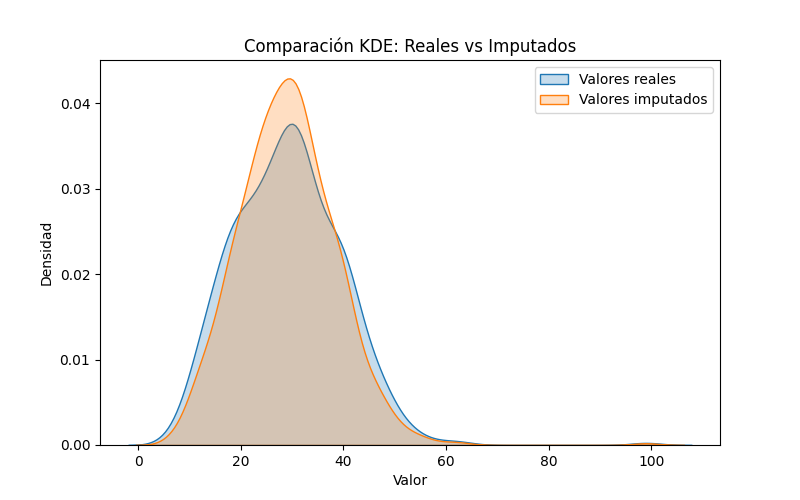
\includegraphics[width=0.75\linewidth]{../Imagenes/Tarea2/Validacion_Original_Imputacion.png}
    \caption{Comparación de densidad (KDE) entre valores originales e imputados mediante KNN para la variable \texttt{Skin\_Fold}.}
    \label{fig:kde_knn}
\end{figure}

Como se observa en la Figura~\ref{fig:kde_knn}, ambas curvas presentan una superposición considerable, lo que indica que el método KNN preserva adecuadamente la forma general de la distribución. No se aprecia un desplazamiento significativo del pico principal ni alteraciones notables en la dispersión de los datos, lo que sugiere que la imputación no introduce sesgos estadísticos relevantes.

Por lo tanto, puede concluirse que el método KNN resultó apropiado para esta variable, manteniendo la coherencia estadística del conjunto de datos.

\subsection{Codificación de Variables}

Posteriormente, se aplicó el proceso de codificación correspondiente a las variables categóricas del conjunto de datos. La codificación transforma las categorías en representaciones numéricas sin alterar la frecuencia original de cada clase.

Se verificó que la transformación mantiene la consistencia de la información, asegurando que la estructura del conjunto de datos permanezca intacta para su posterior análisis.

\subsection{Normalización Min-Max}

Finalmente, se aplicó la normalización Min-Max a la variable \texttt{Skin\_Fold} con el propósito de escalar los valores al intervalo [0,1], utilizando la transformación:

\[
x' = \frac{x - x_{\min}}{x_{\max} - x_{\min}}
\]

Para validar la correcta implementación del método, se graficó la relación entre los valores originales y los valores normalizados.

\begin{figure}[H]
    \centering
    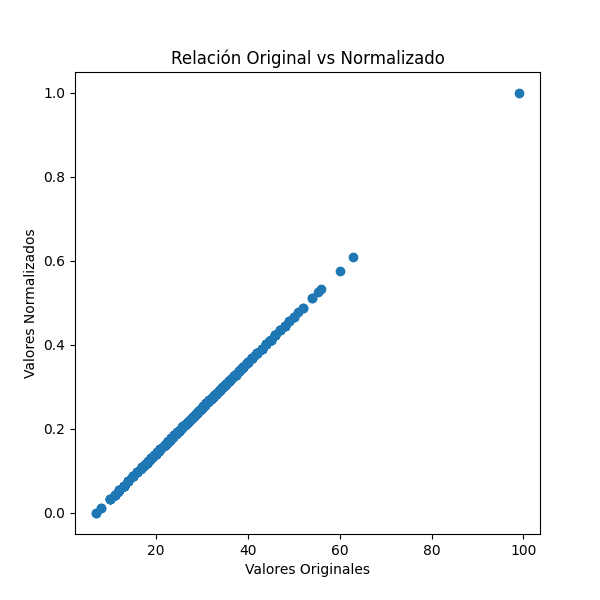
\includegraphics[width=0.75\linewidth]{../Imagenes/Tarea2/Validacion_Normalizacion.png}
    \caption{Relación entre valores originales y valores normalizados mediante Min-Max para la variable \texttt{Skin\_Fold}.}
    \label{fig:normalizacion}
\end{figure}

En la Figura~\ref{fig:normalizacion} se observa que los puntos siguen una tendencia lineal creciente, lo que confirma que la transformación aplicada es lineal. Esto implica que el orden relativo de los datos se conserva y que no se altera la proporción entre los valores originales.

Además, se verificó que el valor mínimo de la variable se transformó en 0 y el valor máximo en 1, cumpliendo con la propiedad fundamental del método Min-Max. En consecuencia, la normalización fue implementada correctamente y permite que la variable pueda ser utilizada en modelos que requieren escalamiento previo.


\section{Conclusión}

El presente trabajo permitió desarrollar e integrar de manera estructurada un proceso completo de preprocesamiento de datos, abarcando desde la gestión de valores faltantes hasta la normalización de variables, utilizando como caso de estudio el conjunto de datos \textit{``Diabetes Dataset with Missing Value for Practice''} disponible en Kaggle.

En primer lugar, se analizaron y aplicaron métodos de imputación, destacando la imputación por media y el método de los vecinos más cercanos (KNN). A partir de la comparación mediante estimación de densidad Kernel (KDE), se observó que el método KNN preserva de mejor manera la forma de la distribución original, manteniendo la variabilidad y reduciendo la introducción de sesgos estadísticos. Esto evidencia la importancia de seleccionar técnicas de imputación que conserven la estructura interna de los datos.

Posteriormente, se realizó el proceso de codificación de variables categóricas, garantizando que la transformación mantuviera la coherencia y frecuencia original de las categorías. Esta etapa permitió adaptar el conjunto de datos para su posible utilización en modelos de aprendizaje automático sin pérdida de información relevante.

En la etapa final, se aplicó la normalización Min-Max, comprobando mediante representación gráfica que la transformación es lineal y conserva el orden relativo de los datos. La validación visual confirmó que el escalamiento fue implementado correctamente, asegurando que las variables se encuentren en un rango adecuado para algoritmos sensibles a la magnitud de los valores.

\printbibliography[title={ Bibliográficas}]
\end{document}